\documentclass[11pt,a4paper]{article}
\usepackage{amsmath}
\usepackage{amsfonts}
\usepackage{amssymb}
\usepackage{makeidx}
\usepackage{graphicx}
\usepackage{wrapfig}
\usepackage{enumerate}
\usepackage{pdfpages}
\usepackage{tocloft}
\usepackage{setspace}
\usepackage{mathtools}
\usepackage{hyperref}
\definecolor{linkcolour}{rgb}{0,0.2,0.6} % Link color
\hypersetup{colorlinks,breaklinks,urlcolor=linkcolour,linkcolor=linkcolour}

\usepackage[left=2cm,right=2cm,top=1.5cm,bottom=1.5cm]{geometry}

\usepackage{xcolor}

\usepackage{fontspec}
\setmainfont{Cambria}

\usepackage{caption}
\captionsetup[figure]{font=small, labelfont={bf}}
\captionsetup[table]{font=small, labelfont={bf}}

\usepackage{float}
\usepackage{multirow}
\usepackage{longtable}

\usepackage[nottoc]{tocbibind}

\newcommand{\spa}{\vspace{1.25em}}
\newcommand{\noi}{\noindent}
\def\dul#1{\underline{\underline{#1}}}
\def\cpt#1#2{{\begin{center}\small\textbf{\textcolor{blue}{Figure #1:}} #2\end{center}}}
\def\tt#1{\texttt{#1}}

% for dots in the content
\usepackage{tocloft}
\renewcommand{\cftsecleader}{\cftdotfill{\cftdotsep}}

\begin{document}
	\begin{titlepage} 
		\begin{center}
		\large{ASSIGNMENT 2}\\
		\vspace{2em}
		\large {CS5691 Pattern Recognition and Machine Learning}
		\vspace{3em}
		
		\rule{0.9\linewidth}{0.5mm} \\[0.4cm]
	    {\Large{\bfseries{CS5691 Assignment 2}}} \\
	    \rule{0.9\linewidth}{0.5mm} \\[3 em]	
	    
	    Team Members: \\
	    \vspace{0.5em}
	   	\def\arraystretch{1.25}
\begin{tabular}{c l}
	\hline
	BE17B007 & N Sowmya Manojna \\
	PH17B010 & Thakkar Riya Anandbhai \\
	PH17B011 & Chaithanya Krishna Moorthy \\
	\hline
\end{tabular}

		\vspace{1em}

		Indian Institute of Technology, Madras\\    
		
		\vspace{5em}    
	    
	    	
\includegraphics[scale = 0.09]{images/iitmlogo.png}
		\end{center}
	\end{titlepage}

{\hypersetup{linkcolor=black}
 \tableofcontents}
\break


\section{Dataset 1A}
\subsection{K-nearest Neighbors Classifier}

The K Nearest Neighbour is a statistically non-parametric model that can be used for regression as well as for classification. It assumes that similar things exist in close proximity.  
\noi
Crucial steps in a K-Nearest Neighbour classifier are:
\begin{itemize}
    \item A distance metric is first specified, the most commonly used metric is the euclidean distance:
    \begin{equation}
        d=||\vec{x_{1}}-\Vec{x_{2}}||
    \end{equation}
    
    where $||.||$ denotes the norm function. Other commonly used distance metrics are the Manhattan distance and cosine similarity. For our application, euclidean distance is used. 
    \item Using the specified distance metric, the distance between the test instance and each training example is evaluated.
    \item The class label that occurs most frequently amongst the nearest k training examples is assigned to the test instance\\
\end{itemize}
\\
Advantages of KNN are:

\begin{itemize}
    \item KNN does not require a training period, it just stores the training dataset and learns from it at the time of making a prediction, hence it is generally much faster than other classification algorithm.
    \item Since the algorithm does not require prior training, new data points can be added seamlessly. 
    \item Easy to implement,the number of parameters are just 2- k and the distance metric to be used 
\end{itemize}
\\
Disdvantages of KNN are:

\begin{itemize}
    \item Computationally expensive for large data sets or high number of features, since the distance is evaluated between test point and all the points in the training data set. 
    \item Sensitive to noisy data and outliers. Generally, increasing the value of k reduces the effect of noise.
\end{itemize}

\subsubsection{Pre-processing}

The data set 1a has 4 unique class labels - {1.0,0.0,2.0,3.0} as shown in the figure. Number of examples corresponding to each class label is 200.
The train data set is of dimension (800,3) while the dev data set is of dimension (120,3).The 3rd column in both data sets is the class label, while the first two columns are the real valued feature vectors- $x_{1} and x_{2}$
\begin{enumerate}
    \item There are no null values in the data sets. 
    \item The rows of dev data set are shuffled and further split into cross-validation and test data in the ratio of 70:30
    \item Range of $x_1$ is (-11,11) and range of $x_2$ is (-12,7). Since the ranges are almost similar, no feature scaling is required.  
\end{enumerate}

\subsubsection{Model performance for varying values of k}

The model was evaluated for k values = {1,7,15}. We find that irrespective of the value of hyper-parameter k, the model obtained an accuracy of 1 over training data, cross-validation data as well as the test data. Since model performance is best irrespective of k, the accuracy table, confusion matrix and decision boundary plot are all evaluated using k=1 as to minimize the run time. 
\noindent
The accuracy table and confusion matrix are: 
\def\arraystretch{1.25}
\begin{center}
\begin{longtable}{l l l l l}
\hline
\hline
\textbf{k-value} & \textbf{Train accuracy} & \textbf{Cross-validation accuracy} & \textbf{Test Accuracy}\\
\hline
\hline
1 & 1.00 & 1.00 & 1.00 \\
7 & 1.00 & 1.00 & 1.00 \\
15 & 1.00 & 1.00 & 1.00 \\

\hline
\end{longtable}
\setcounter{table}{0}
\captionof{table}{Accuracy table for data set 1a- knn classifier}
\end{center}

\begin{figure}[H]
    \centering
    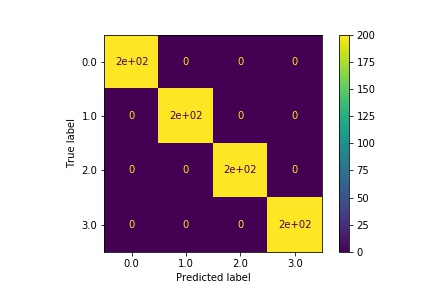
\includegraphics[scale=0.5]{images/1a_cm_knn_train.jpg}
    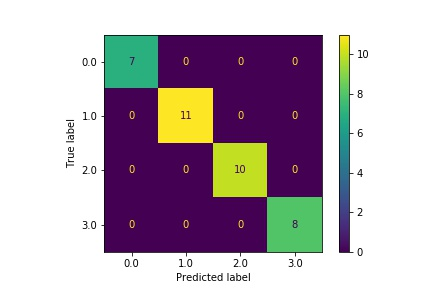
\includegraphics[scale=0.5]{images/1a_cm_knn_test.jpg}
    \caption{Confusion matrix for k=1, Train and Test data set on left and right respectively}
    \label{fig:1a_cm_knn}
\end{figure}

\subsubsection{Decision region plot with training data superposed}

\begin{figure}[H]
    \centering
    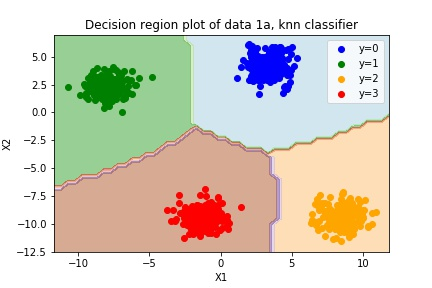
\includegraphics[scale=0.5]{images/1a_knn_decision_region.jpg}
    \caption{Decision region superimposed with training data set}
    \label{fig:1a_decreg_knn}
\end{figure}

The decision boundary obtained (with k=1) is linear in form. 


\subsection{Naive-Bayes classifier with Gaussian distribution for each class}

The Bayes Classifiers are probabilistic classifiers based on the Bayes theorem:

\begin{equation}
\label{eqn nb}
    p(y_{i}/\vec{x})=\frac{p(\vec{x}/y_{i})*p(y_{i})}{p(\vec{x})}
\end{equation}
\\
Here, \\ 
$p(y_{i})$ : prior probability for $y=y_{i}$. \\
$p(\vec{x}/y_{i})$ : Class conditional probability density function or class conditional likelihood function. \\
$p(y_{i}/\vec{x})$ : Posterior probability for $y=y_{i}$ given $\vec{x}$.\\
$p(\vec{x})$ : Evidence or normalization factor.
\noindent
\\
Equation \ref{eqn nb} can be re-written as:
\begin{equation} \label{normalized_nb}
    p(y_{i}/\vec{x})=\frac{p(\vec{x}/y_{i})*p(y_{i})}{\sum_{i}p(\vec{x}/y_{i})*p(y_{i})}
\end{equation}

\\
\noindent
Hence, the probability that $\vec{x}$ belongs to the class $y_{i}$ is $\propto$ $p(\vec{x}/y_{i})*p(y_{i})$. \\
\noi
Step-wise approach:
\begin{itemize}
    \item $p(y_{i})$ is calculated from the train data set, for data set 1a, we find that all the classes have equal prior probability.
    \item The probability $p(\vec{x}/y_{i})$ can be calculated by various parametric and non-parametric means. For data set 1a, we use parametric means as described later.
    \item $p(y_{i}/\vec{x})$ is calculated for all the classes using equation \ref{normalized_nb}.
    \item The class label with maximum posterior probability is chosen as the class label for $\vec{x}$.
\end{itemize}
\subsubsection{Same Covariance Matrix ($\sigma^2I$)}
\subsubsection{Same Covariance Matrix ($C$)}
\subsubsection{Different Covariance Matrix}

\break
\section{Dataset 1B}
\subsection{K-nearest Neighbors Classifier}
\subsection{Bayes Classifier, GMM, full covariance}
\subsubsection{Equations}
Th initialization is done as follows for each class:
\begin{itemize}
    \itemsep0em
    \item Cluster initialization is using \tt{kmeans} clustering.
    \item The relative number of points in each cluster $N_q$ and weightage $w_q$ for each cluster is calculated.
    \item The responsibility $\gamma_{n,q}$ is then calculated, followed by mean $\mu_q$ and covariance $C_q$ is calculated.
\end{itemize}

\noi
The parameters are then updated sequentially through the:
\begin{itemize}
    \itemsep0em
    \item Expectation-step: $\gamma_{n,q}$ is updated.
    \item Maximization-step: $\mu_q$, $C_q$, $N_q$ and $w_q$ are updated.
\end{itemize}

\noi
The stopping criterion used is $\Delta(\text{likelihood})<\tt{tol}$. The \tt{tol} we considered is $10^{-5}$.\\

\noi
Based on the accuracies obtained on the training, validation and test dataset, the best $q_i$ for the three classes has been chosen as $5$. The accuracies obtained in tabular format is as follows:
\begin{table}[H]
\centering
\begin{tabular}{l l l l}
\hline
\hline
\textbf{Number of Clusters/Class (Q)} & \textbf{Train Accuracy} & \textbf{Validation Accuracy} & \textbf{Test Accuracy}\\
\hline
\hline
2 & 0.968333 & 0.952381 & 0.925926 \\
3 & 0.983333 & 0.968254 & 1.000000 \\
4 & 0.996667 & 0.984127 & 1.000000 \\
5 & 0.998333 & 1.000000 & 1.000000 \\
6 & 0.996667 & 1.000000 & 1.000000 \\
7 & 0.998333 & 1.000000 & 1.000000 \\
8 & 0.996667 & 1.000000 & 1.000000 \\
9 & 0.996667 & 1.000000 & 1.000000 \\
\hline
\end{tabular}
\caption{Variation of accuracy across hyperparameter values on the training, validation and test set using the GMM model with full covariance matrix on Dataset 1B}
\label{tab:1b_full}
\end{table}



\subsubsection{Training and Validation Accuracy}
The training and validation accuracies obtained for varying $q_i$ for each class is as follows:
\begin{figure}[H]
    \hspace{-2em}
    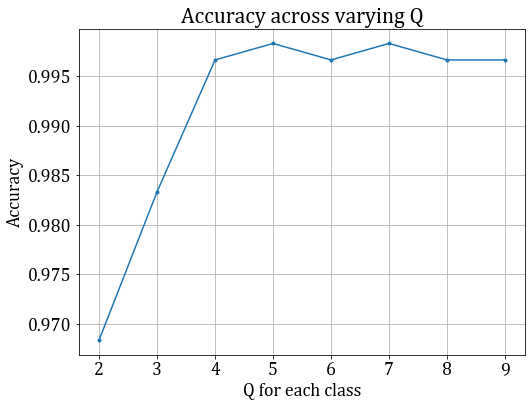
\includegraphics[scale=0.5]{images/1b_full_train.png}
    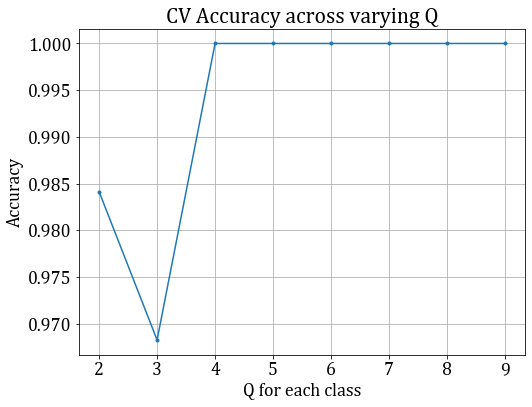
\includegraphics[scale=0.5]{images/1b_full_val.png}
    \caption{Training and Validation accuracy across $q_i$, on the left and right respectively}
\end{figure}

\subsubsection{Testing Accuracy}
The testing accuracy obtained for varying $q_i$ for each class is as follows:
\begin{figure}[H]
    \centering
    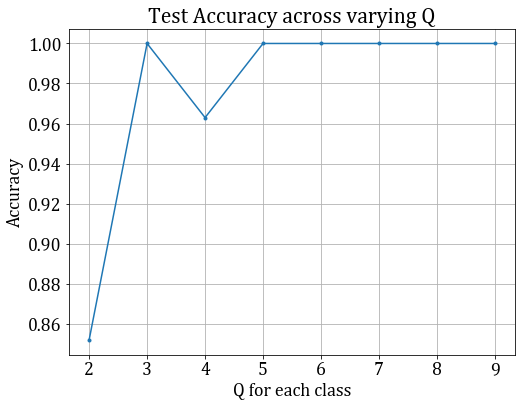
\includegraphics[scale=0.45]{images/1b_full_test.png}
    \caption{Testing accuracy across $q_i$}
\end{figure}

\subsubsection{Contour Maps and Decision Surfaces}
The contour maps and decision surfaces obtained, with $q_i=5$ are as follows:
\begin{figure}[H]
    \hspace{-1em}
    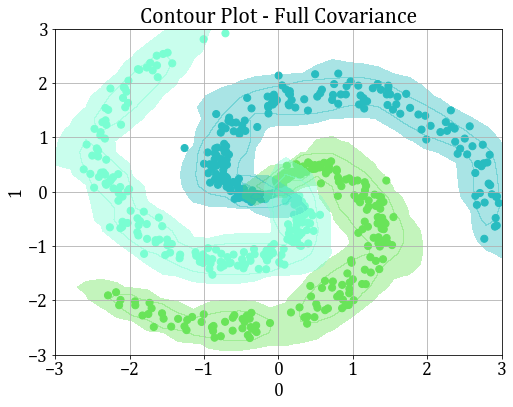
\includegraphics[scale=0.45]{images/1b_full_contours.png}
    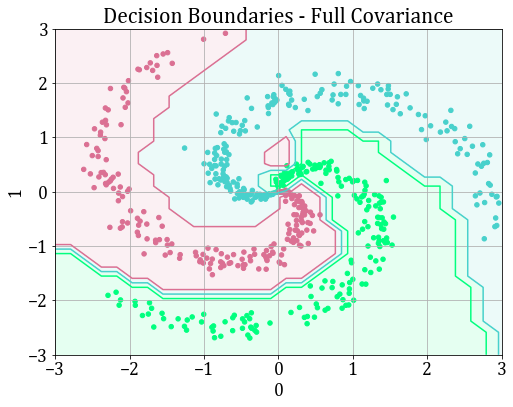
\includegraphics[scale=0.45]{images/1b_full_decision_surfaces.png}
    \caption{Contour Maps, Decision Surfaces obtained for $q_i=5$, on the left and right respectively.}
\end{figure}

\begin{figure}[H]
    \centering
    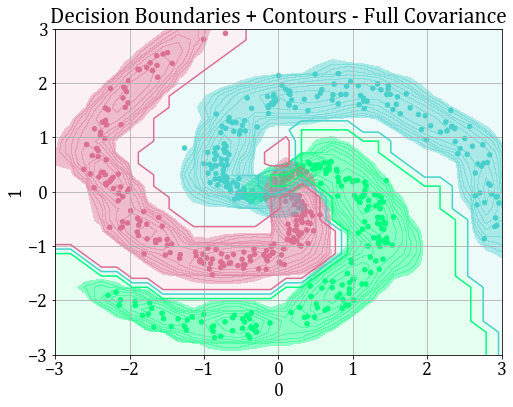
\includegraphics[scale=0.45]{images/1b_full_ds_contours.png}
    \caption{Overlap plot of the decision surface and contours.}
\end{figure}


\subsection{Bayes Classifier, GMM, diagonal covariance}
\subsubsection{Training and Validation accuracy}
Gaussian multi-modal training function (with threshold of the increment in total log-likelihood functions as 0.01 since there was no significant improvement for a smaller threshold than this) with diagonal covariance matrix over the hyperparameter values of the number of gaussian components Q = {2,3,4,5,6,7,8,9} to estimate the parameters - $\mu_q$, $C_q$, $N_q$ and $w_q$ for each gaussian component - and predict the classes of the training data (train.csv) and cross-validation (70\% of dev.csv), we get the table \ref{tab:cv1b}
\begin{table}[H]
\centering
\begin{tabular}{l l l }
\hline
\hline
\textbf{Hyperparameter Value (Q)} &  \textbf{Accuracy on CV data} &  \textbf{Accuracy on Training data}  \\
\hline
\hline
2 & 0.873 & 0.9166\\
3 & 0.920 & 0.976\\
4 & 0.968 & 0.9966\\
5 & 0.984 & 1.0\\
6 & 0.984 & 0.986\\
7 & 0.984 & 0.991\\
8 & 0.984 & 0.9916\\
9 & 0.984 & 0.9916\\
\hline
\end{tabular}
\caption{Variation of Accuracy across Hyperparameter values on the validation data using the GMM model with diagonal covariance matrix on Dataset 1B}
\label{tab:cv1b}
\end{table}


\begin{figure}[H]
    \centering
    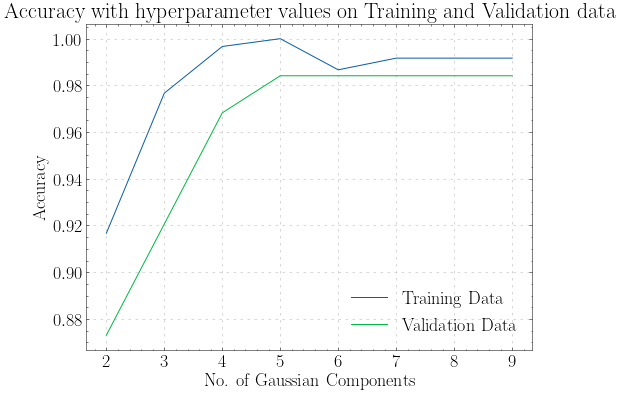
\includegraphics[scale=0.5]{images/acc_1b.png}
    \caption{Plot of Hyperparameter value Vs Accuracy using the GMM model with diagonal covariance matrix on Dataset 1B}
    \label{fig:acc1bGMMdiag}
\end{figure}
\subsubsection{Best model output}
As we can see in the tables and figure \ref{fig:acc1bGMM}, the best accuracy is when the number of Gaussian components is 5. Using the parameters of the model for 5 gaussian components and predicting for the test dataset (30\% of dev.csv), the accuracy obtained was \textbf{1.0}.\\
The confusion matrices for the training and test datasets using the best model are tables \ref{tab:conf_train1b} and \ref{tab:conf_test1b}.\\
\begin{table}[H]
\centering
\begin{tabular}{|l|l|l|l|}
\hline
&0&1&2\\
\hline
0&200&0&0\\
\hline
1&0&200&0\\
\hline
2&0&0&200\\
\hline
\end{tabular}
\caption{Confusion Matrix for training data 1B}
\label{tab:conf_train1b}
\end{table}


\begin{table}[]
    \centering
    
        \begin{tabular}{|l|l|l|l|}
            \hline
            &0&1&2\\
            \hline
            0&9&0&0\\
            \hline
            1&0&10&0\\
            \hline
            2&0&0&8\\
            \hline
 \end{tabular}

\caption{Confusion Matrix for test data 1B}
    \label{tab:conf_train1b}
\end{table}

The decision region plot for the best model is figure \ref{fig:dec1bGMMdiag}
\begin{figure}[H]
    \centering
    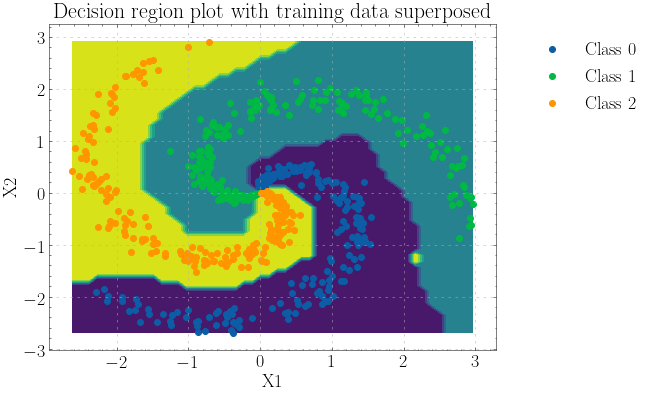
\includegraphics[scale = 0.5]{images/decisionReg_ds2.png}
    \caption{Decision region plot for Bayesian GMM model using diagonal covariance matrix and 5 gaussian components on dataset 1B}
    \label{fig:dec1bGMMdiag}
\end{figure}
\subsection{Bayes Classifier, KNN}

\break
\section{Dataset 2A}
\subsection{Bayes Classifier, GMM, full covariance}
\subsection{Bayes Classifier, GMM, diagonal covariance}
\subsubsection{Training and Validation Accuracy}
The accuracy obtained on training the data 2A on GMM model with diagonal covariance matrix is as in table \ref{tab:acc2a}. The plot of the same is in figure \ref{fig:acc2adiag}. The tolerence used was 1e-3.
\begin{table}[H]
\centering
\begin{tabular}{l l l l}
\hline
\hline
\textbf{# Clusters/Class (Q)} & \textbf{Training Accuracy} & \textbf{Validation Accuracy}\\
\hline
\hline
2 & 0.509 & 0.350\\
3 & 0.525 & 0.404\\
4 & 0.574 & 0.436\\
5 & 0.627 & 0.420\\
6 & 0.6491 & 0.418\\
\hl{7} & \hl{0.663} & \hl{0.440}\\
8 & 0.689 & 0.371\\
9 & 0.692 & 0.413\\
10 & 0.718 & 0.427\\
11 & 0.735 & 0.396\\
12 & 0.754 & 0.393\\
13 & 0.770 & 0.434\\
14 & 0.783 & 0.388\\
\hline
\end{tabular}
\caption{Variation of accuracy across hyperparameter values on the training and validation using the GMM model with diagonal covariance matrix on Dataset 2A. }
\label{tab:acc2a}
\end{table}



\begin{figure}[H]
    \centering
    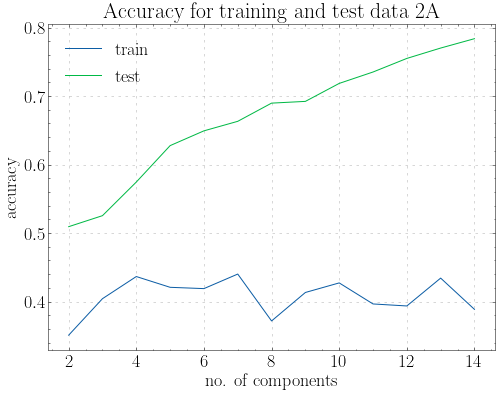
\includegraphics[scale = 0.5]{acc_2a.png}
    \caption{Accuracy for training and validation set for 2A}
    \label{fig:acc2adiag}
\end{figure}

\subsection{Best model on test data}
The highest accuracy on validation data set is for 7 gaussian components. Applying this model to predict the test data, we get an accuracy of \textbf{0.37}. The confusion matrices for this model on training and test data are tables \ref{tab:conf_train2a} and \ref{tab:conf_test2a}.
\begin{table}[H]
\centering
\begin{tabular}{|l|l|l|l|l|l|}
\hline
 & 0 & 1 & 2 & 3 & 4 \\
\hline
0 & 147 & 8 & 21 & 22 & 35 \\
\hline
1 & 7 & 156 & 7 & 13 & 14 \\
\hline
2 & 39 & 5 & 165 & 30 & 45 \\
\hline
3 & 25 & 7 & 20 & 190 & 24 \\
\hline
4 & 33 & 6 & 36 & 32 & 143 \\
\hline
\end{tabular}
\caption{Confusion Matrix for training data 2A}
\label{tab:conf_train2a}
\end{table}

\begin{table}[]
    \centering
\begin{tabular}{|l|l|l|l|l|l|}
\hline
&0&1&2&3&4\\
\hline
0&37&4&11&12&7\\
\hline
1&5&25&6&3&4\\
\hline
2&12&10&27&19&20\\
\hline
3&9&8&12&40&21\\
\hline
4&10&5&15&8&23\\
\hline
\end{tabular}
\caption{Confusion Matrix for test data 2A}
    \label{tab:conf_train2a}
\end{table}


\break
\section{Dataset 2B}
\subsection{Bayes Classifier, GMM, full covariance}
\subsection{Bayes Classifier, GMM, diagonal covariance}


\end{document}
